\documentclass[12pt]{article}
\usepackage{titling}
\usepackage{graphicx}
\usepackage{caption}
\usepackage{helvet}
\usepackage{hyperref}
\usepackage{bookmark}
\usepackage{framed}
\usepackage{listings}
\usepackage{mdframed}
\usepackage{sectsty}
\usepackage{tikz}
\newcommand{\abs}[1]{\left|#1\right|}

\renewcommand{\lstlistingname}{}

% Define font size and family for sections
\sectionfont{\fontsize{10}{12}\selectfont\renewcommand{\familydefault}{\sfdefault}}
\subsectionfont{\fontsize{10}{12}\selectfont\renewcommand{\familydefault}{\sfdefault}}
\subsubsectionfont{\fontsize{10}{12}\selectfont\renewcommand{\familydefault}{\sfdefault}}
\paragraphfont{\fontsize{10}{12}\selectfont\renewcommand{\familydefault}{\sfdefault}}
\subparagraphfont{\fontsize{10}{12}\selectfont\renewcommand{\familydefault}{\sfdefault}}
\renewcommand{\familydefault}{\rmdefault} % Reset default to Roman for title page

\usepackage[utf8]{inputenc}
\usepackage{amsmath}
\usepackage{hyperref}

\lstset{
    language=Matlab,
    basicstyle=\ttfamily\footnotesize,
    keywordstyle=\color{blue},
    commentstyle=\color{green},
    stringstyle=\color{red},
    frame=single,
    breaklines=true,
    keepspaces=true,
    showspaces=false,
    showstringspaces=false
}


\begin{document}

% Prima pagina
\begin{titlepage}
    \centering
    {\Huge \textbf{Università degli Studi di Padova} \par}
    \vspace{1cm}
    \begin{figure}[h!]
        \centering
        \includegraphics[width=0.6\textwidth]{Immagini/Logo_Università_Padova.png}
    \end{figure}
    \vspace{1.5cm}
    {\LARGE \textbf{Relazione per:} \par}
    {\Huge Progetto 2 Matlab \par}
    \vfill
    \textbf{Realizzata da:} \par
    Riccardo Berengan, matricola 2080041 \par
    Michele Dioli, matricola 2077629 \par
    Gabriele Di Pietro, matricola 2010000 \par
    \vspace{0.5cm}
\end{titlepage}
    % Change font and size for the rest of the document
    \renewcommand{\familydefault}{\sfdefault} % Set default to sans serif
    \fontsize{10}{12}\selectfont
    % Pagina introduzione
    \newpage
    \section{Introduzione}
    Gli autovalori sono le soluzioni dell'equazione $det(A-\lambda I) = 0$. 
    L'autospazio è il sottospazio vettoriale generato da tutti i vettori autovalori $\lambda$, insieme al vettore nullo.\\ \textit{Esempio:}
    \begin{align*}
        A &= \begin{bmatrix}
            4 & 2 \\
            1 & 3 \\
        \end{bmatrix}
    \end{align*}
    $det(A-\lambda I) = det\begin{bmatrix}
        4-\lambda & 2 \\
        1 & 3-\lambda \\
    \end{bmatrix} \iff (\lambda - 5)(\lambda-2) = 0 \iff \lambda_1 = 5 \lambda_2 = 2$\\
    Molteplicità geometrica è la dimensione dell'autospazio associato ad un autovalore quindi $\abs{n - \text{rk}(A - \lambda I)}$
    Molteplicità geometrica è la dimensione dell'autospazio associato ad un autovalore quindi $|n - rk(A - \lambda I)|$
    \section{Calcolo}
    \subsection{Funzione Multigeo}
    Per il calcolo contiamo gli elementi "nulli" \textit{(minori di una tolleranza)} sulla matrice $U$ ottenuta dalla fattorizzazione $LU$. Lo si può fare perchè:
    Una riga nulla in $U$ significa che il sistema lineare di $(A-\lambda I)x = 0$ ha soluzione libera, una riga nulla non dipende dalle altre righe della matrice, le righe nulle indicano che ci sono dipendenze lineari tra le righe.
    Contiamo quindi gli elementi in diagonale che sono maggiori di una tolleranza, contando così il rango della matrice, lo sottraiamo alla dimensione della matrice e otteniamo la dimensione dell'autospazio dell'autovalore che coincide con la molteplicità geometrica.
    \subsection{Funzione myobjective}
    La funzione \texttt{myobjective} calcola la funzione $f$ e la funzione $g$ a partire da uno scalare $z$ e da una matrice $A$ quadrata.\\
    Come prima cosa calcoliamo la matrice $B = A - zI$ e poi tramite fattorizzazione LU usando \texttt{lu(B)} in Matlab che restituisce la matrice $U$ triangolare superiore e la matrice $L$ triangolare inferiore ed infine la matrice $P$ di permutazione. \\
    $P=\pm1$ in base al numero di permutazioni effettuate, da qui calcoliamo il determinante di P. Trovato questo calcoliamo il determinante di $B$ come $det(P) \cdot \prod_{i=1}^{n} U_{ii}$, dove $U_{ii}$ sono gli elementi sulla diagonale di $U$. $f = det(B)$\\
    La funzione dopodichè calcola l'inverso della matrice $B$  e calcola $g$ come l'inverso della traccia \textit{(somma degli elementi sulla diagonale)} di $B$.
    \newpage

    \subsection{Funzione Multialg}
    Consideriamo il polinomio con $m$ molteplicità algebrica $f(x)=(x-\lambda)^m g(x)$ e il metodo di Newton $x_{n+1}=x_n - \frac{f(x_n)}{f'(x_n)}$ per trovare le radici di $g(x)$.
    Analizziamo la velocità di convergenza di $f(x)=(x-\lambda)^{m-1} g(x) + (x-\lambda)^m g'(x)$\\
    $f'(x) = 0 \iff x = \lambda$, $m \geq 1$ non è subito alla radice $m(x-\lambda)^{m-1}$ è responsabile per la velocità di convergenza, quindi il metodo di Newton applicato ad una radice di molteplicità $m\geq 1$ ha una velocità lineare non più quadratica.\\
    Abbiamo che la stima dell'errore è ridotta dipendentemente dalla molteplicità della radice $|x_{n+1}-\lambda| \approx |x_n - \lambda|^{\frac{m-1}{m}}$\\
    $\frac{m-1}{m}$ è la velocità di convergenza\\ \textit{(Newton vicino a radici multiple $\Rightarrow |e_{n+1}| \approx C|e_n|^{\frac{m-1}{m}}$)}\\
    Calcoliamo l'autovalore con il metodo di Newton, iteriamo fino a un numero di iterazioni e/o per aver raggiunto una tolleranza sensata. Applichiamo Newton al polinomio caratteristico $f(\lambda) = det(A-\lambda I) \Rightarrow \lambda_{n+1} = \lambda_n - \frac{f(\lambda_n)}{f'(\lambda_n)}$. Troviamo così il valore dell'autovalore.
    Per calcolare la molteplicità algebrica basta dividere l'autovalore per il polinomio caratteristico, e vedere quante volte lo posso fare prima di ottenere un valore di zero.
    \section{Test}
    \subsection{File \texttt{main.m}}
    Il main permette di definire una matrice di test tramite la modifica del vettore \texttt{lambda} e  di modificare il punto iniziale per il metodo di newton \texttt{lO} e il parametro della tolleranza \texttt{toll}.\\
    La matrice per i test viene creata tramite la modifica del parametro \texttt{lambda} da qui viene invocata una funzione \texttt{creaJacob} che prende in input \texttt{lambda} e restituisce la matrice in forma diagonale a blocchi di Jordan, poi viene creata una matrice $Q$ tramite \texttt{Q = orth(randn(n))} che genera una matrice ortogonale, ed infine viene calcolata la matrice $A$ usando la struttura $A=Q^tJQ$\\
    \newpage
    \subsection{File \texttt{test.m}}
    Il programma \texttt{test.m} esegue una serie di test per verificare la correttezza delle funzioni \texttt{multialg} e \texttt{multigeo}. Queste funzioni sono utilizzate per calcolare gli autovalori di una matrice e le loro rispettive molteplicità algebriche e geometriche.
    Il programma definisce una serie di casi di test, ciascuno con una matrice di autovalori specificata dal vettore \texttt{lambda}, un punto iniziale per il metodo di Newton \texttt{lO}, e una tolleranza \texttt{toll}.
    \begin{lstlisting}[language=Matlab, frame=single, caption={Test Cases}, captionpos=b]         
TestCases = {
    struct('lambda', [1,1,1,1,1,4,4,4,4,4,4,4], 'lO', 3.8, 'toll', 1e-4),
    struct('lambda', [1, 1.01, 1.02, 5, 5.01, 5.02, 10, 10.001, 10.002, 10.003], 'lO', 10.1, 'toll', 1e-4),
    struct('lambda', [1, 1.01, 1.02, 5, 5.01, 5.02, 10, 10.001, 10.002, 10.003], 'lO', 1.0125, 'toll', 1e-4),
    struct('lambda', [1,1,1,4,5,6], 'lO', 3.5, 'toll', 1e-4),
    struct('lambda', [1,1,1,4,5,6], 'lO', 3.9, 'toll', 1e-4),
    struct('lambda', [1,1,1,4,5,6,4], 'lO', 3.9, 'toll', 1e-4),
    struct('lambda', [1,1,1,4,5,6,4,4], 'lO', 3.5, 'toll', 1e-4),
    struct('lambda', [1,1,1,4,5,6,4,4,4], 'lO', 3.7, 'toll', 1e-4), 
    struct('lambda', [1,1,1,4,5,6,4,4,4,4], 'lO', 3.3, 'toll', 1e-4), 
    struct('lambda', [1,1,1,4,5,6,4,4,4], 'lO', 3.7, 'toll', 1e-4),
    struct('lambda', [1,1,1,4,5,6,4,4,4,4], 'lO', 3.5, 'toll', 1e-4),
    struct('lambda', [1,1,1,4,5,6,4,4,4,4,4], 'lO', 4.3, 'toll', 1e-4), 
    struct('lambda', [1,1,1,4,5,6,4,4,4,4,4], 'lO', 3.5, 'toll', 1e-4), 
    struct('lambda', [1,1,1,4,5,6,4,4,4,4,4,4], 'lO', 3.4, 'toll', 1e-4),
    struct('lambda', [4,4,4,4,4,4,4,4], 'lO', 0., 'toll', 1e-4),
};
    \end{lstlisting}
    \newpage
\subsubsection{Esecuzione dei test}
Per ogni caso di test, il programma esegue i seguenti passaggi:
    \begin{enumerate}
        \item Stampa il numero del test e i valori di \texttt{lambda}, \texttt{lO}, e \texttt{toll}.
        \item Crea una matrice diagonale \texttt{J} con i valori di \texttt{lambda} e aggiunge 1 agli elementi fuori diagonale per gestire le molteplicità.
        \item Genera una matrice ortogonale \texttt{Q} e calcola la matrice \texttt{A} come \texttt{A = Q' * J * Q}.
        \item Utilizza la funzione \texttt{multialg} per calcolare un autovalore \texttt{l} e la sua molteplicità algebrica \texttt{m}.
        \item Se il metodo di Newton converge, calcola la molteplicità geometrica \texttt{k} dell'autovalore utilizzando la funzione \texttt{multigeo}.
        \item Stampa i risultati del test, inclusi l'autovalore calcolato, la molteplicità algebrica e geometrica, e un messaggio di convergenza.
    \end{enumerate}
    Il programma fornisce un'analisi dettagliata dei risultati di ciascun test, permettendo di verificare l'accuratezza e l'efficacia delle funzioni implementate.
    \newpage
\begin{lstlisting}[language=Matlab, frame=single, caption={Esecuzione dei test}, captionpos=b]
for testID = 1:length(TestCases)
    fprintf('\nExecuting Test %d...\n', testID);    
    lambda = TestCases{testID}.lambda;
    fprintf('[%s]\n', sprintf('%g ', lambda));
    lO = TestCases{testID}.lO;
    fprintf('lO = %d\n', TestCases{testID}.lO);
    toll = TestCases{testID}.toll;
    fprintf('toll = %d\n', TestCases{testID}.toll);
    J = diag(lambda);
    for i = 2:length(lambda)
        if J(i,i) == J(i-1,i-1)
            J(i-1,i) = 1;
        end
    end
    n = length(lambda);
    Q = orth(randn(n)); 
    A = Q' * J * Q;
    A1 = A;
    disp(J);     
    it = 5;
    maxit = 50;
    [l, m, flag] = multialg(A, lO, toll, it, maxit);
    if flag == 1
        fprintf('Newton convergence.\nCalculated eigenvalue: %f\nEstimated algebraic multiplicity: %d\n', l, m);
        l1 = round(l);
        toll = 1e-6;
        k = multigeo(A1, l1, toll);
        fprintf('Geometric multiplicity of %f: %d\n', l1, k);
    else
        fprintf('Non-convergent Method.\n');
    end
    linea = 50;
    fprintf('%s\n', repmat('-', 1, linea));
end
\end{lstlisting}
\newpage
\subsubsection{Terminal output}
Per comodità ci riserviamo di stampare solo un test case, gli altri sono simili.
    \begin{framed}
    \begin{verbatim}
Executing Test 14...
[1 1 1 4 5 6 4 4 4 4 4 4 ]
lO = 3.400000e+00
toll = 1.000000e-04
     1     1     0     0     0     0     0     0     0     0     0     0
     0     1     1     0     0     0     0     0     0     0     0     0
     0     0     1     0     0     0     0     0     0     0     0     0
     0     0     0     4     0     0     0     0     0     0     0     0
     0     0     0     0     5     0     0     0     0     0     0     0
     0     0     0     0     0     6     0     0     0     0     0     0
     0     0     0     0     0     0     4     1     0     0     0     0
     0     0     0     0     0     0     0     4     1     0     0     0
     0     0     0     0     0     0     0     0     4     1     0     0
     0     0     0     0     0     0     0     0     0     4     1     0
     0     0     0     0     0     0     0     0     0     0     4     1
     0     0     0     0     0     0     0     0     0     0     0     4
        
Newton convergence.
Calculated eigenvalue: 4.000005
Estimated algebraic multiplicity: 7
Geometric multiplicity of 4.000000: 2
--------------------------------------------------
    \end{verbatim}
    \end{framed}
    \begin{center}
        \textbf{3: Output di un test case}
    \end{center}
    \newpage
    \begin{figure}[htbp]
        \begin{tikzpicture}
            \node[anchor=east,inner sep=0] (img1) at (0,0) {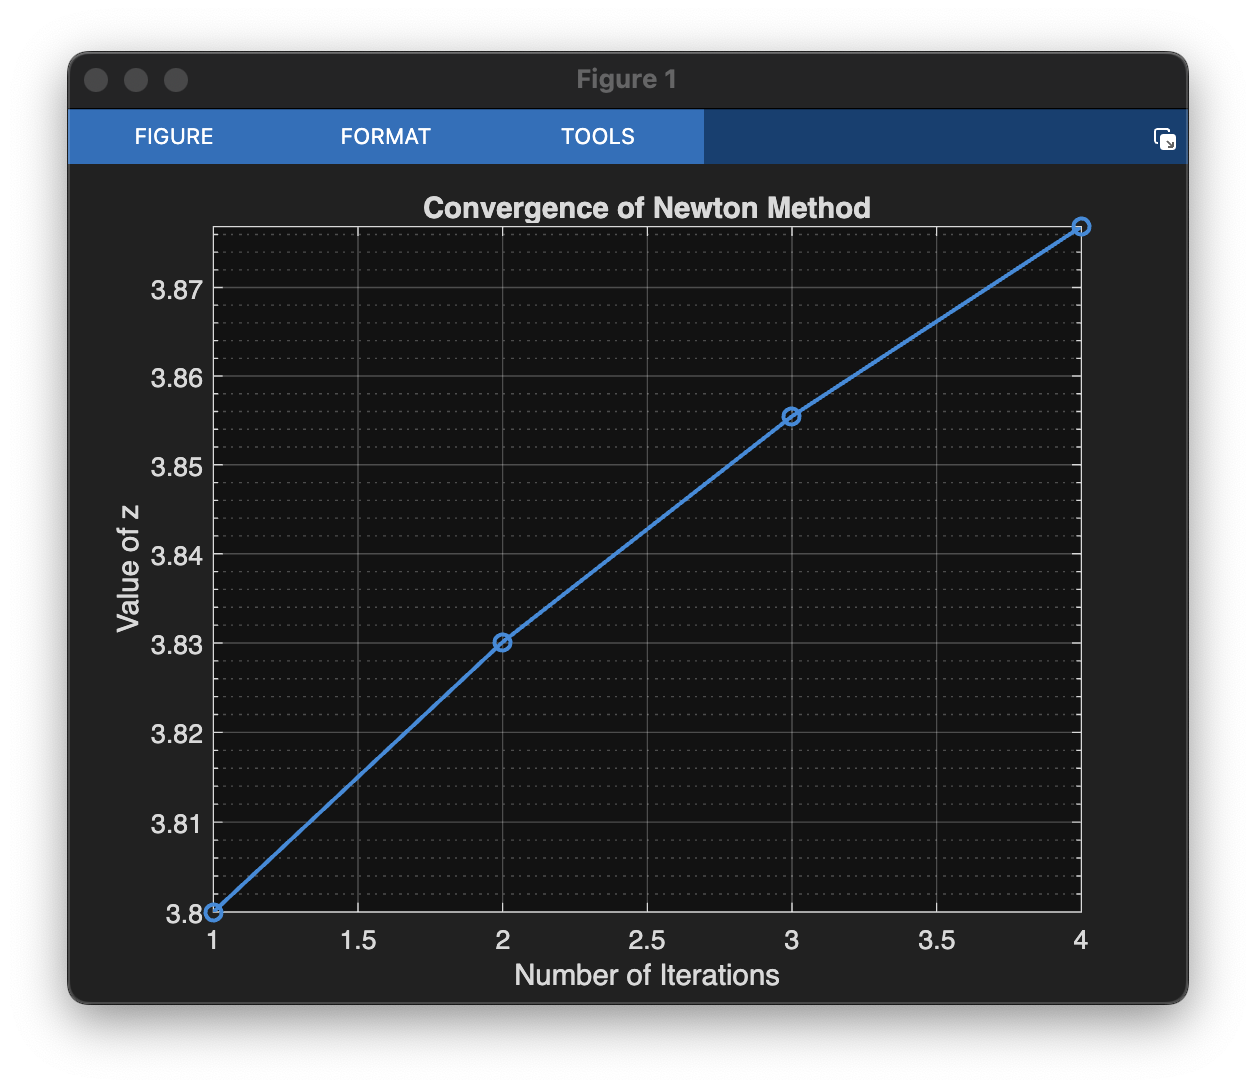
\includegraphics[width=0.5\textwidth]{Immagini/figure1.png}};
            \node[anchor=west,inner sep=0] (img2) at (0.1,0) {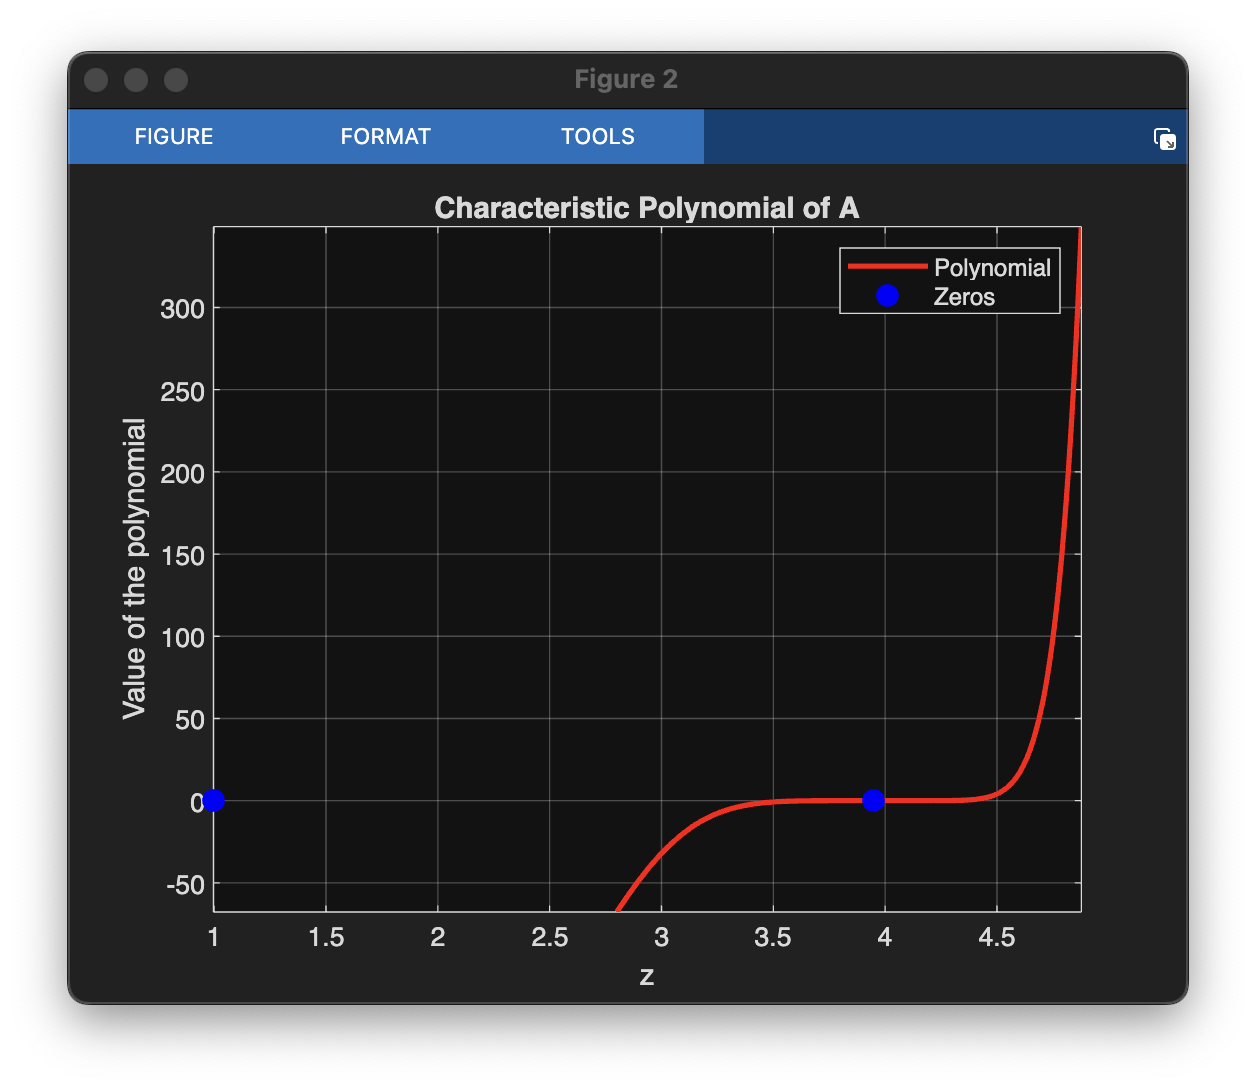
\includegraphics[width=0.5\textwidth]{Immagini/figure2.png}};
        \end{tikzpicture}
            \caption{\textit{Convergenza del metodo di Newton e polinomio di A}}
    \end{figure}
Verranno anche mostrate su grafici apparte sia la convergenza del metodo di Newton, sia il polinomio di A.

    \section{Conclusioni}
    Possiamo concludere che il software prodotto gestisce bene il problema e può trovare autovalori anche con stime iniziali lontani, infatti il metodo di Newton converge anche con stime iniziali molto distanti (\textit{ad esempio}, \texttt{lO}$= 3.5$ per $\lambda = 4$). \\ 
    Il software è stato testato con matrici di varie dimensioni e con molteplicità algebriche e geometriche diverse, e in tutti i casi il metodo di Newton converge, a meno che non si scelga un punto iniziale molto distante dall'autovalore da trovare\\
\end{document}
